\documentclass[tikz]{standalone}
\usepackage{pgffor}

\begin{document}
    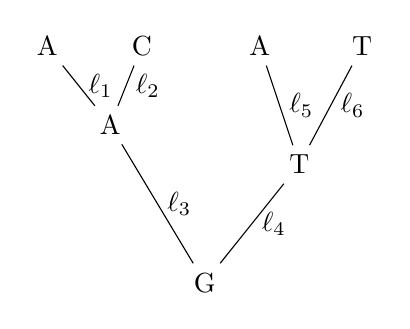
\begin{tikzpicture}
        \foreach \x/\y/\n/\l/\j/\k in {-2/2/a/A,-0.8/2/b/C,0.7/2/c/A,2/2/d/T}{
            \node[] (\n) at (\x,\y) {\l};
        }
        \foreach \x/\y/\n/\l in {-1.2/1/lnode/A,1.2/0.5/rnode/T,0/-1/r/G}{
            \node[] (\n) at (\x,\y) {\l};
        }
        \foreach \m/\n/\l in {a/lnode/{$\ell _1$},b/lnode/{$\ell _2$},c/rnode/{$\ell _5$},d/rnode/{$\ell _6$},lnode/r/{$\ell _3$},rnode/r/{$\ell _4$}}{
            \draw[] (\m) -- node[right]{\l} (\n);
        }
    \end{tikzpicture}
\end{document}